Troopers may use vehicles, such as motorcycles and hoverbikes, for enhanced mobility.

\paragraph*{Vehicle Card}

The unit card shows the current capabilities of a vehicle and tracks damage.
A unit card can be formatted in any way so long as it contains all the essential information.
Below is a sample unit card for a basic motorcyle.

\begin{figure}[!h]
  \centering
  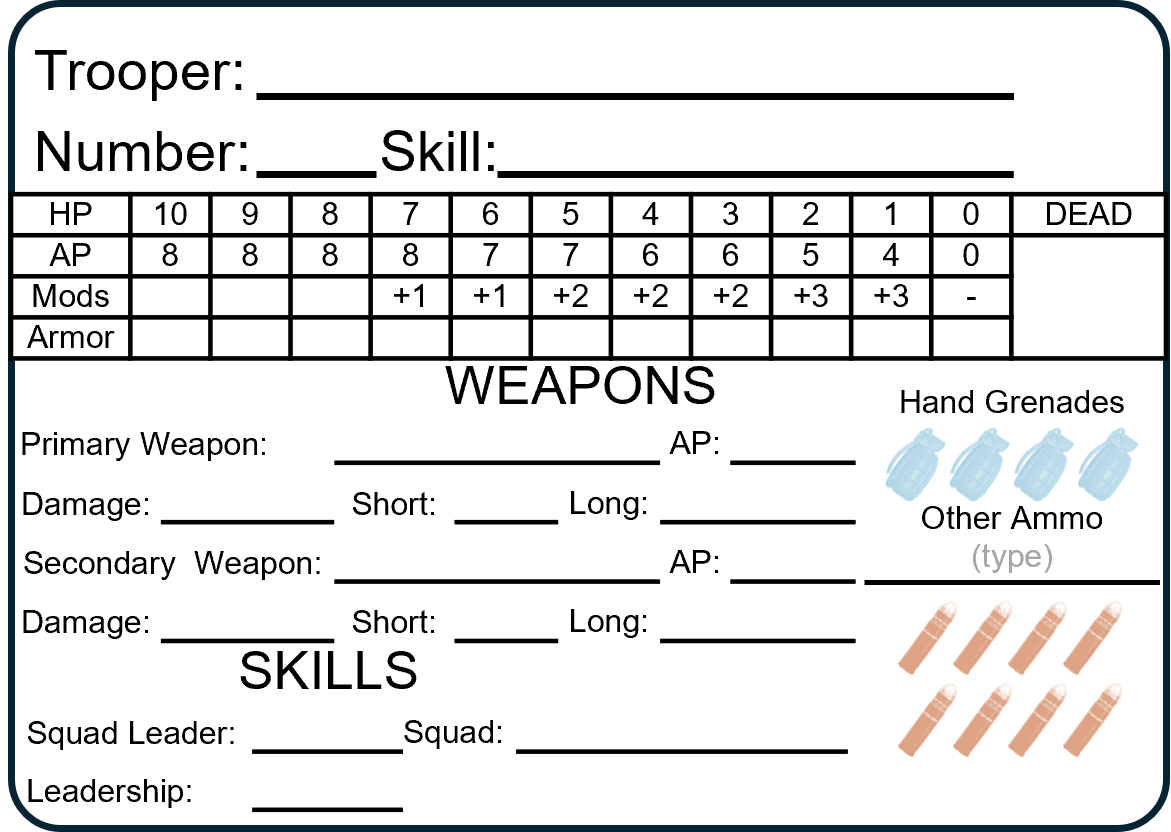
\includegraphics[alt='Sample Regular Trooper', width=5.63in, height=4in]{img/RegularTrooper.png}
  \caption*{Basic Motorcycle Vehicle Unit Card}
\end{figure}

Damage to the vehicle is tracked in the HP section.
HP cells are labeled by their HP value, from highest to lowest, 12 to 0, from left to right.
HP cells are fully crossed out when the vehicle takes standard damage (X).
Vehicles ignore bludgeoning damage (\textbackslash).
The current HP of the vehicle is given by the first cell to the right of the lowest fully marked HP cell.

If the vehicle's armor value is given by in the armor section.
Subtract this value from the total amount of standard damage (X) done to the vehicle prior to assigning the damage to a location.
The armor may reduce the damage to 0.

The maximum valid movement mode for the vehicle is given in the movement mode section.
Use the value in the column corresponding to the vehicle's current HP.
For example, if the vehicle has 5 HP, then it can only use the minimum or cruse movement modes.

Similarly, the modifier section tracks the current modifier for the vehicle's target numbers based upon current HP.
This modifier only applies to vehicle control checks and attacks made with weapons mounted to the vehicle.
For example, if the vehicle has 5 HP, then add +2 to all target numbers.

The weapons section list the weapons mounted on the vehicle, along with their orientation, damage values, and range brackets.

\paragraph*{Movement}

In order to use a vehicle, a trooper must first mount the vehicle and turn it on.
The vehicle stays on until turned off.

\begin{table}[!h]
\ifthenelse{\not \equal{\outworldsMode}{mode-web}}{\fontfamily{Montserrat-LF}}{\small}\selectfont
\centering
\newcolumntype{R}[1]{>{\raggedleft\let\newline\\\arraybackslash\hspace{0pt}}m{#1}}
\begin{tabular}{!{\Vline{1pt}} m{9em} !{\Vline{1pt}} R{4.5em} !{\Vline{1pt}}}
\Hline{1pt}
\rowcolor{black!30}  \bfseries{Action} & \bfseries{AP Cost} \\
\Hline{1pt}
Mount/Dismount & 2  \\
Turn on/off    & 1  \\
\Hline{1pt}
\end{tabular}
\caption*{Vehicle AP Costs}
\end{table}

Once a trooper is on the vehicle, they must select a movement mode for the turn.
A trooper can only select a movement mode if they have sufficient remaining AP for that movement mode and the vehicle currently supports that movement mode.

\begin{table}[!h]
\ifthenelse{\not \equal{\outworldsMode}{mode-web}}{\fontfamily{Montserrat-LF}}{\small}\selectfont
\centering
\newcolumntype{R}[1]{>{\raggedleft\let\newline\\\arraybackslash\hspace{0pt}}m{#1}}
\begin{tabular}{!{\Vline{1pt}} m{10em} !{\Vline{1pt}} R{4.5em} !{\Vline{1pt}}}
\Hline{1pt}
\rowcolor{black!30}  \bfseries{Movement Mode} & \bfseries{AP Used} \\
\Hline{1pt}
Minimum & 1  \\
Cruise  & 4  \\
Max     & 7  \\
\Hline{1pt}
\end{tabular}
\caption*{Vehicle Movement Modes}
\end{table}

The trooper must use the exact number of AP given by the movement mode to move the vehicle, unless the vehicle is brought to a full stop.
Accelerating from a full stop costs 1 AP and decelerating to a full stop costs 2 AP.
The vehicle card says how many dots the vehicle moves for each AP spent to move.
The vehicle also moves this number of dots while starting from a full stop or going to a full stop.

\begin{table}[!h]
\ifthenelse{\not \equal{\outworldsMode}{mode-web}}{\fontfamily{Montserrat-LF}}{\small}\selectfont
\centering
\newcolumntype{R}[1]{>{\raggedleft\let\newline\\\arraybackslash\hspace{0pt}}m{#1}}
\begin{tabular}{!{\Vline{1pt}} m{10em} !{\Vline{1pt}} R{4.5em} !{\Vline{1pt}}}
\Hline{1pt}
\rowcolor{black!30}  \bfseries{Action} & \bfseries{AP Cost} \\
\Hline{1pt}
Start from full stop & 1  \\
Go to full stop      & 2  \\
Move                 & 1  \\
\Hline{1pt}
\end{tabular}
\caption*{Vehicle Movement AP Costs}
\end{table}

While moving, the vehicle may spend AP to turn.
A vehicle must move forward by at least 1 dot before turning.
The front of the vehicle stays in place while the rear of the vehicle swings to a new dot for turning.
Since a 60 degree (1 dot) turn costs no AP to execute, it is the only turn that can be executed during the minimum movement mode.

\begin{table}[!h]
\ifthenelse{\not \equal{\outworldsMode}{mode-web}}{\fontfamily{Montserrat-LF}}{\small}\selectfont
\centering
\newcolumntype{R}[1]{>{\raggedleft\let\newline\\\arraybackslash\hspace{0pt}}m{#1}}
\begin{tabular}{!{\Vline{1pt}} m{8em} !{\Vline{1pt}} R{4.5em} !{\Vline{1pt}}}
\Hline{1pt}
\rowcolor{black!30}  \bfseries{Action} & \bfseries{AP Cost} \\
\Hline{1pt}
 60 degree turn & 0  \\
120 degree turn & 1  \\
180 degree turn & 2  \\
\Hline{1pt}
\end{tabular}
\caption*{Vehicle Turning Movement AP Costs}
\end{table}

When executing a 120 or 180 degree turn, the trooper must make a control check.
A control check is a 2D6 check with the target number set by the chart below, will any applicable modifiers for damage to the trooper and the vehicle.

\begin{table}[!h]
\ifthenelse{\not \equal{\outworldsMode}{mode-web}}{\fontfamily{Montserrat-LF}}{\small}\selectfont
\centering
\newcolumntype{R}[1]{>{\raggedleft\let\newline\\\arraybackslash\hspace{0pt}}m{#1}}
\begin{tabular}{!{\Vline{1pt}} m{8em} !{\Vline{1pt}} R{8em} !{\Vline{1pt}}}
\Hline{1pt}
\rowcolor{black!30}  \bfseries{Action} & \bfseries{Target Number} \\
\Hline{1pt}
 60 degree turn & -  \\
120 degree turn & 6  \\
180 degree turn & 9  \\
\Hline{1pt}
\end{tabular}
\caption*{Vehicle Turning Control Check}
\end{table}

Decelerating to a full stop while using the cruise or maximum movement modes also requires a control check.
A trooper may incorporate a turn into the deceleration to a full stop, but this increases the difficulty of the control check.

\begin{table}[!h]
\ifthenelse{\not \equal{\outworldsMode}{mode-web}}{\fontfamily{Montserrat-LF}}{\small}\selectfont
\centering
\newcolumntype{R}[1]{>{\raggedleft\let\newline\\\arraybackslash\hspace{0pt}}m{#1}}
\begin{tabular}{!{\Vline{1pt}} m{8em} !{\Vline{1pt}} R{8em} !{\Vline{1pt}}}
\Hline{1pt}
\rowcolor{black!30}  \bfseries{Action} & \bfseries{Target Number} \\
\Hline{1pt}
 no turn        & 4  \\
 60 degree turn & 4  \\
120 degree turn & 6  \\
180 degree turn & 8  \\
\Hline{1pt}
\end{tabular}
\caption*{Vehicle Deceleration Control Check}
\end{table}

When a vehicle enters an enemy firing arc, resolve the attack immediately.
The enemy unit may target either the vehicle or the trooper, but not both.
If the damage to the vehicle makes the current movement mode invalid or damage to the trooper leaves insufficient AP to complete the current movement mode, then they automatically wipe out as if they had failed a control check.

\paragraph*{Vehicle Damage}

When applying damage to a vehicle, first subtract the vehicle's armor value from the total damage.
Then, roll 2D6.
This is the initial cell to apply damage in.
Starting with the initial cell, mark off the number of cells given by the modified damage value, skipping any previously marked cells.

\paragraph*{Wipeout}

If a trooper fails a control check, then they wipe out.
If the vehicle was attempting to turn, then set the rear of the vehicle as if it had completed a 60 degree shallower turn.
For example, if trooper wiped out while executing a 120 degree turn, then set the rear of the vehicle as if it had completed a 60 degree turn.
The vehicle then skids along the ground in a straight line from this point.
If the vehicle was using the cruise movement mode, then it skids the number of dots given by 1 AP of movement, and if the vehicle was using the maximum movement mode, then it skids the number of dots given by 2 AP of movement.
If the vehicle hits an object while skidding, then stop the skid immediately and apply ramming damage to the vehicle and trooper.

After wiping out, it costs 3 AP for a trooper to climb out from underneath a vehicle and and additional 3 AP to lift the vehicle to an upright position.

\begin{table}[!h]
\ifthenelse{\not \equal{\outworldsMode}{mode-web}}{\fontfamily{Montserrat-LF}}{\small}\selectfont
\centering
\newcolumntype{R}[1]{>{\raggedleft\let\newline\\\arraybackslash\hspace{0pt}}m{#1}}
\begin{tabular}{!{\Vline{1pt}} m{8em} !{\Vline{1pt}} R{4.5em} !{\Vline{1pt}}}
\Hline{1pt}
\rowcolor{black!30}  \bfseries{Action} & \bfseries{AP Cost} \\
\Hline{1pt}
Crawl out    & 3  \\
Lift vehicle & 3  \\
\Hline{1pt}
\end{tabular}
\caption*{Vehicle Wipeout Costs}
\end{table}

\paragraph*{Combat}

A trooper may make four types of attacks while on a vehicle - ramming, melee, movement fire, and standard fire.
All of these attacks, except standard fire, occur during the movement of the vehicle.

When a vehicle's front is in the same dot as an enemy trooper or vehicle, the vehicle makes a ramming attack.
Apply the ramming damage to both the vehicle and the enemy unit, then make a control check with a base target number of 6.
On a failed control check, the trooper wipes out, as above.

\begin{table}[!h]
\ifthenelse{\not \equal{\outworldsMode}{mode-web}}{\fontfamily{Montserrat-LF}}{\small}\selectfont
\centering
\newcolumntype{R}[1]{>{\raggedleft\let\newline\\\arraybackslash\hspace{0pt}}m{#1}}
\begin{tabular}{!{\Vline{1pt}} m{10em} !{\Vline{1pt}} R{4.5em} !{\Vline{1pt}}}
\Hline{1pt}
\rowcolor{black!30}  \bfseries{Movement Mode} & \bfseries{Damage} \\
\Hline{1pt}
Minimum & 1  \\
Cruise  & 3  \\
Max     & 5  \\
\Hline{1pt}
\end{tabular}
\caption*{Vehicle Ramming Damage}
\end{table}

When a vehicle's front is adjacent to enemy trooper or vehicle, the trooper on the vehicle may make a melee attack.
The trooper's active melee weapon does additional damage based upon the movement mode of the vehicle.
Apply the melee damage to the enemy trooper, then make a control check with a base target number of 6.
On a failed control check, the trooper wipes out, as above.

\begin{table}[!h]
\ifthenelse{\not \equal{\outworldsMode}{mode-web}}{\fontfamily{Montserrat-LF}}{\small}\selectfont
\centering
\newcolumntype{R}[1]{>{\raggedleft\let\newline\\\arraybackslash\hspace{0pt}}m{#1}}
\begin{tabular}{!{\Vline{1pt}} m{10em} !{\Vline{1pt}} R{4.5em} !{\Vline{1pt}}}
\Hline{1pt}
\rowcolor{black!30}  \bfseries{Movement Mode} & \bfseries{Damage} \\
\Hline{1pt}
Minimum & +0X  \\
Cruise  & +1X  \\
Max     & +2X  \\
\Hline{1pt}
\end{tabular}
\caption*{Vehicle Melee Damage}
\end{table}

The trooper may make attacks with the movement fire rules with their current active weapon or any weapons mounted on the vehicle.
As with standard movement fire, add 2 to the target number.
Burst fire weapons may be fired multiple times if the trooper has sufficient AP, and the vehicle may continue moving after firing.
If the trooper is using an explosive weapon, the explosive damage is still resolved after all troopers have moved, as usual.

After movement, the trooper may spend AP to establish a firing arc.
Any weapons mounted on the vehicle automatically establish a appropriate firing arc at a 0 AP cost.
